% Pengaturan ukuran teks dan bentuk halaman dua sisi
\documentclass[12pt]{report}

% Pengaturan ukuran halaman dan margin
\usepackage[a4paper,top=30mm,left=30mm,right=20mm,bottom=25mm]{geometry}

% Pengaturan ukuran spasi
\usepackage[singlespacing]{setspace}

% Pengaturan caption untuk tabel
\usepackage{caption}

% Judul dokumen
\title{Proposal Tugas Akhir ITS}
\author{Musk, Elon Reeve}

% Pengaturan detail pada file PDF
\usepackage[pdfauthor={\@author},bookmarksnumbered,pdfborder={0 0 0}]{hyperref}


% Pengaturan ukuran indentasi
\setlength{\parindent}{2em}

% Package lainnya
\usepackage{changepage}
\usepackage{etoolbox} % Mengubah fungsi default

% Pengaturan jenis karakter
\usepackage[utf8]{inputenc}

\usepackage[style=apa, backend=biber]{biblatex}
\usepackage{enumitem} % Pembuatan list
\usepackage{lipsum} % Pembuatan template kalimat
\usepackage{graphicx} % Input gambar
\usepackage{longtable} % Pembuatan tabel
\usepackage[table,xcdraw]{xcolor} % Pewarnaan tabel
\usepackage{eso-pic} % Untuk menggunakan background image di halaman
\usepackage{txfonts} % Font times
\usepackage{changepage} % Pembuatan teks kolom
\usepackage{multicol} % Pembuatan kolom ganda
\usepackage{multirow} % Pembuatan baris ganda
\usepackage{tabularx} % Untuk mengatur kolom, seperti grid pada CSS
\usepackage{wrapfig}

% Pengaturan format daftar isi, daftar gambar, dan daftar tabel
\usepackage{tocloft}
\setlength{\cftbeforechapskip}{1.5ex}
\setlength{\cftbeforesecskip}{1.5ex}
\setlength{\cftbeforetoctitleskip}{0cm}
\setlength{\cftbeforeloftitleskip}{0cm}
\setlength{\cftbeforelottitleskip}{0cm}
\renewcommand{\cfttoctitlefont}{\hfill\Large\bfseries} % command untuk membuat heading bold dan besar
\renewcommand{\cftaftertoctitle}{\hfill}
\renewcommand{\cftloftitlefont}{\hfill\Large\bfseries}
\renewcommand{\cftafterloftitle}{\hfill}
\renewcommand{\cftlottitlefont}{\hfill\Large\bfseries}
\renewcommand{\cftafterlottitle}{\hfill}

% Definisi untuk "Hati ini sengaja dikosongkan"
\patchcmd{\cleardoublepage}{\hbox{}}{
  \thispagestyle{empty}
  \vspace*{\fill}
  \begin{center}\textit{[Halaman ini sengaja dikosongkan]}\end{center}
  \vfill}{}{}

  % Pengaturan penomoran halaman
\usepackage{fancyhdr}
\fancyhf{}
\renewcommand{\headrulewidth}{0pt}
\pagestyle{fancy}
\fancyfoot[C,CO]{\thepage}
\patchcmd{\chapter}{plain}{fancy}{}{}
\patchcmd{\chapter}{empty}{plain}{}{}

% Pengaturan format judul bab
\usepackage{titlesec}
\renewcommand{\thesection}{\thechapter.\arabic{section}}
\titleformat{\chapter}[hang]{\centering\bfseries\Large}{BAB\ \arabic{chapter}\ }{0ex}{\vspace{0ex}\centering}
\titleformat*{\section}{\large\bfseries}
\titleformat*{\subsection}{\normalsize\bfseries}
\titlespacing{\chapter}{0ex}{0ex}{4ex}
\titlespacing{\section}{0ex}{1ex}{0ex}
\titlespacing{\subsection}{0ex}{0.5ex}{0ex}
\titlespacing{\subsubsection}{0ex}{0.5ex}{0ex}
\setcounter{secnumdepth}{3} % Untuk memberi penomoran pada \subsubsection

\counterwithin{figure}{chapter}
\counterwithin{table}{chapter}

% Mengganti figure dan table menjadi gambar dan tabel
\renewcommand{\figurename}{Gambar}
\renewcommand{\tablename}{Tabel}

% Tambahkan format tanda hubung yang benar di sini
\hyphenation{
  ro-ket
  me-ngem-bang-kan
  per-hi-tu-ngan
}

% Menambahkan resource daftar pustaka
\addbibresource{pustaka/pustaka.bib}

% Isi keseluruhan dokumen
\begin{document}
  % Nomor halaman pembuka dimulai dari sini
  \pagenumbering{roman}

  % Atur ulang penomoran halaman
  \setcounter{page}{1}

  % Sampul Bahasa Indonesia
  \newcommand\covercontents{sampul/konten-id.tex}
  \AddToShipoutPictureBG*{
  \AtPageLowerLeft{
    % Ubah nilai berikut jika posisi horizontal background tidak sesuai
    \hspace{-3.25mm}

    % Ubah nilai berikut jika posisi vertikal background tidak sesuai
    \raisebox{0mm}{
      
\includegraphics[width=\paperwidth,height=\paperheight]{sampul/gambar/sampul-luar-tipis.png}
    }
  }
}

% Menyembunyikan nomor halaman
\thispagestyle{empty}

% Pengaturan margin untuk menyesuaikan konten sampul
\newgeometry{
  top=65mm,
  left=30mm,
  right=30mm,
  bottom=20mm
}

\begin{flushleft}

  % Pemilihan font sans serif
  \sffamily

  % Pemilihan font bold
  \fontseries{bx}
  \selectfont
  \begin{spacing}{1.5}
    \input{\covercontents}
  \end{spacing}

\end{flushleft}

\restoregeometry


  % Sampul Bahasa Inggris
  \renewcommand\covercontents{sampul/konten-en.tex}
  \AddToShipoutPictureBG*{
  \AtPageLowerLeft{
    % Ubah nilai berikut jika posisi horizontal background tidak sesuai
    \hspace{-3.25mm}

    % Ubah nilai berikut jika posisi vertikal background tidak sesuai
    \raisebox{0mm}{
      
\includegraphics[width=\paperwidth,height=\paperheight]{sampul/gambar/sampul-luar-tipis.png}
    }
  }
}

% Menyembunyikan nomor halaman
\thispagestyle{empty}

% Pengaturan margin untuk menyesuaikan konten sampul
\newgeometry{
  top=65mm,
  left=30mm,
  right=30mm,
  bottom=20mm
}

\begin{flushleft}

  % Pemilihan font sans serif
  \sffamily

  % Pemilihan font bold
  \fontseries{bx}
  \selectfont
  \begin{spacing}{1.5}
    \input{\covercontents}
  \end{spacing}

\end{flushleft}

\restoregeometry


  % Lembar pengesahan
  \begin{center}
	\large
  \textbf{LEMBAR PENGESAHAN}
\end{center}

% Menyembunyikan nomor halaman
\thispagestyle{empty}

\begin{center}
  % Ubah kalimat berikut dengan judul tugas akhir
  \textbf{KALKULASI ENERGI PADA ROKET LUAR ANGKASA BERBASIS \emph{ANTI-GRAVITASI}}
\end{center}

\begingroup
  % Pemilihan font ukuran small
  \small

  \begin{center}
    % Ubah kalimat berikut dengan pernyataan untuk lembar pengesahan
    \textbf{PROPOSAL TUGAS AKHIR} \\
    Diajukan untuk memenuhi salah satu syarat memperoleh gelar
    Sarjana Teknik pada 
    Program Studi S-1 Teknik Dirgantara \\
    Departemen Teknik Dirgantara \\
    Fakultas Teknik Dirgantara \\
    Institut Teknologi Sepuluh Nopember
  \end{center}

  \begin{center}
    % Ubah kalimat berikut dengan nama dan NRP mahasiswa
    Oleh: \textbf{Elon Reeve Musk} \\
    NRP. 0123 20 4000 0001
  \end{center}

  \begin{center}
    Disetujui oleh Tim Penguji Proposal Tugas Akhir:
  \end{center}

  \begingroup
    % Menghilangkan padding
    \setlength{\tabcolsep}{0pt}

    \noindent
    \begin{tabularx}{\textwidth}{X c}
      % Ubah kalimat-kalimat berikut dengan nama dan NIP dosen pembimbing pertama
      Nikola Tesla, S.T., M.T.          & (Pembimbing) \\
      NIP: 18560710 194301 1 001        & \\
      &  \\
      &  \\
      % Ubah kalimat-kalimat berikut dengan nama dan NIP dosen pembimbing kedua
      Wernher von Braun, S.T., M.T.     & (Ko-Pembimbing) \\
      NIP: 19230323 197706 1 001        & \\
      &  \\
      &  \\
      % Ubah kalimat-kalimat berikut dengan nama dan NIP dosen penguji pertama
      Dr. Galileo Galilei, S.T., M.Sc.  & (Penguji I) \\
      NIP: 15640215 164201 1 001        & \\
      &  \\
      &  \\
      % Ubah kalimat-kalimat berikut dengan nama dan NIP dosen penguji kedua
      Friedrich Nietzsche, S.T., M.Sc.  & (Penguji II) \\
      NIP: 18441015 190008 1 001        & \\
      &  \\
      &  \\
      % Ubah kalimat-kalimat berikut dengan nama dan NIP dosen penguji ketiga
      Alan Turing, ST., MT.             & (Penguji III) \\
      NIP: 19120623 195406 1 001        & \\
    \end{tabularx}
  \endgroup

  \vspace{4ex}

  \begin{center}
    % Ubah text dibawah menjadi tempat dan tanggal
    \textbf{SURABAYA} \\
    \textbf{Mei, 2077}
  \end{center}
\endgroup

  \newpage

  % Lembar pengesahan
  \begin{center}
	\large
  \textbf{APPROVAL SHEET}
\end{center}

% Menyembunyikan nomor halaman
\thispagestyle{empty}

\begin{center}
  % Ubah kalimat berikut dengan judul tugas akhir
  \textbf{\emph{ANTI-GRAVITY} BASED ENERGY CALCULATION ON OUTER SPACE ROCKETS}
\end{center}

\begingroup
  % Pemilihan font ukuran small
  \small

  \begin{center}
    % Ubah kalimat berikut dengan pernyataan untuk lembar pengesahan
    \textbf{FINAL PROJECT PROPOSAL} \\
    Submitted to fulfill one of the requirements for obtaining a degree
    Bachelor of Engineering at 
    Undergraduate Study Program of Aerospace Engineering \\
    Department of Aerospace Engineering \\
    Faculty of Aerospace Technology \\
    Sepuluh Nopember Institute of Technology
  \end{center}

  \begin{center}
    % Ubah kalimat berikut dengan nama dan NRP mahasiswa
    By: \textbf{Elon Reeve Musk} \\
    NRP. 0123 20 4000 0001
  \end{center}

  \begin{center}
    Approved by Final Project Proposal Examiner Team:
  \end{center}

  \begingroup
    % Menghilangkan padding
    \setlength{\tabcolsep}{0pt}

    \noindent
    \begin{tabularx}{\textwidth}{X c}
      % Ubah kalimat-kalimat berikut dengan nama dan NIP dosen pembimbing pertama
      Nikola Tesla, S.T., M.T.          & (Advisor) \\
      NIP: 18560710 194301 1 001        & \\
      &  \\
      &  \\
      % Ubah kalimat-kalimat berikut dengan nama dan NIP dosen pembimbing kedua
      Wernher von Braun, S.T., M.T.     & (Co-Advisor) \\
      NIP: 19230323 197706 1 001        & \\
      &  \\
      &  \\
      % Ubah kalimat-kalimat berikut dengan nama dan NIP dosen penguji pertama
      Dr. Galileo Galilei, S.T., M.Sc.  & (Examiner I) \\
      NIP: 15640215 164201 1 001        & \\
      &  \\
      &  \\
      % Ubah kalimat-kalimat berikut dengan nama dan NIP dosen penguji kedua
      Friedrich Nietzsche, S.T., M.Sc.  & (Examiner II) \\
      NIP: 18441015 190008 1 001        & \\
      &  \\
      &  \\
      % Ubah kalimat-kalimat berikut dengan nama dan NIP dosen penguji ketiga
      Alan Turing, ST., MT.             & (Examiner III) \\
      NIP: 19120623 195406 1 001        & \\
    \end{tabularx}
  \endgroup

  \vspace{4ex}

  \begin{center}
    % Ubah text dibawah menjadi tempat dan tanggal
    \textbf{SURABAYA} \\
    \textbf{May, 2077}
  \end{center}
\endgroup

  \newpage

  % Abstrak
  \begin{center}
  \large
  \textbf{PENGEMBANGAN \emph{DEAD RECKONING} BERBASIS \emph{DEEP LEARNING}  
  UNTUK NAVIGASI JALAN DENGAN SENSOR BERBIAYA RENDAH IMU 
  DAN MIKROKONTROLER STM}
\end{center}
\addcontentsline{toc}{chapter}{ABSTRAK}
% Menyembunyikan nomor halaman
\thispagestyle{empty}

\begin{flushleft}
  \setlength{\tabcolsep}{0pt}
  \bfseries
  \begin{tabular}{ll@{\hspace{6pt}}l}
  Nama Mahasiswa / NRP&:& Muhammad Rafie Azmi / 0721194000077\\
  Departemen&:& Teknik Komputer FTEIC - ITS\\
  Dosen Pembimbing&:& 1. Dion Hayu Fandiantoro, S.T., M.T.\\
  & & 2. Arief Kurniawan, S.T., M.T.\\
  \end{tabular}
  \vspace{4ex}
\end{flushleft}
\textbf{Abstrak}

% Isi Abstrak
Pengguna yang berpindah dari titik P0 ke titik P1 dapat diilustrasikan berada dalam elips keper- cayaan 95 persen berpusat pada P1 dengan sumbu AB, ditentukan oleh heading akurasi sensor, 
dan CD, ditentukan oleh sensor kecepatan ketepatan. Melakukan Dead Reckoning menggunakan Recurrent Neural Network, jaringan perlu dilatih pada kumpulan data input yang terdiri dari posisi 
kendaraan sebelumnya dan data sensorik yang dikumpulkan selama periode waktu tertentu, dan label output yang sesuai yang mewakili posisi kendaraan saat ini. Ada banyak aplikasi potensial 
untuk menggunakan Convolutional Neural Network untuk perhitungan mati, termasuk kendaraan otonom, drone, dan robot seluler lainnya. Kemampuan untuk secara akurat memperkirakan posisi 
kendaraan saat ini berdasarkan posisi sebelumnya dan data sensorik dapat sangat penting untuk navigasi dan lokalisasi di lingkungan di mana sinyal GPS. Dari penelitian yang akan dilakukan, 
diharapkan pengendara yang sudah dilengkkapi alat dapat menentukan sebuah posisi mereka tanpa perlu mengkhawatirkan medan perlitasan yang dilewati (seperti underground and forest) dengan 
penerapan metode Dead Reckoning berbasis Deep Learning sehingga menghasilkan luaran berupa navigasi secara Real Time dengan akurasi tinggi.



\vspace{2ex}
\noindent
\textbf{Kata Kunci: \emph{Dead Reckoning, RNN, Global Position System}}
  \newpage

  \begin{center}
  \large
  \textbf{DEVELOPMENT OF DEEP LEARNING-BASED DEAD RECKONING 
  FOR ROAD NAVIGATION 
  WITH IMU LOW-COST SENSORS AND STM MICROCONTROLLERS}
\end{center}
% Menyembunyikan nomor halaman
\thispagestyle{empty}

\begin{flushleft}
  \setlength{\tabcolsep}{0pt}
  \bfseries
  \begin{tabular}{lc@{\hspace{6pt}}l}
  Student Name / NRP&: &Muhammad Rafie Azmi / 07211940000077\\
  Department&: &Computer Engineering FTEIC - ITS\\
  Advisor&: &1. Dion Hayu Fandiantoro, S.T., M.T.\\
  & & 2. Arief Kurniawan, S.T., M.T.\\
  \end{tabular}
  \vspace{4ex}
\end{flushleft}
\textbf{Abstract}

% Isi Abstrak
Users moving from point P0 to point P1 can be illustrated to be in an ellipse
95 percent confidence centered on P1 with AB axis, determined by heading accuracy
sensors, and CDs, are determined by the accuracy speed sensor.Doing Dead Reckoning
using the Recurrent Neural Network, the network needs to be trained on an input data set that
consists of the vehicle's previous position and sensory data collected during the period
specific time, and corresponding output labels that represent the current position of the vehicle. Exist
many potential applications for using Convolutional Neural Network for perhitu-
ngan die, including autonomous vehicles, drones and other mobile robots.Ability to
accurately estimate the current position of the vehicle based on its previous position and data
Sensory can be critical for navigation and localization in environments where GPS signals.From the research that will be carried out, it is expected that motorists who have been equipped with da-
Pat determines their position without worrying about the terrain of the perlitasan
bypassed (such as underground and forest) with the application of the Dead Reckoning-based method
Deep Learning so as to produce outputs in the form of navigation in Real Time with accuracy
tall.

\vspace{2ex}
\noindent
\textbf{Keywords: \emph{Dead Reckoning, RNN, Global Position System}}
  \newpage

  \begin{spacing}{1.5}
    % Daftar isi
    \renewcommand*\contentsname{DAFTAR ISI}
    \addcontentsline{toc}{chapter}{\contentsname}
    \tableofcontents
    \newpage

    % Daftar gambar
    \renewcommand*\listfigurename{DAFTAR GAMBAR}
    \addcontentsline{toc}{chapter}{\listfigurename}
    \listoffigures
    \newpage

    % Daftar tabel
    \renewcommand*\listtablename{DAFTAR TABEL}
    \addcontentsline{toc}{chapter}{\listtablename}
    \listoftables
    \newpage
  \end{spacing}

  % Nomor halaman isi dimulai dari sini
  \pagenumbering{arabic}

  % Konten pendahuluan
  \chapter{PENDAHULUAN}

\section{Latar Belakang}

% Ubah paragraf-paragraf berikut sesuai dengan LATAR BELAKANG dari tugas akhir
Saat ini metode penentuan posisi suatu titik di permukaan bumi mengalami kemajuan teknologi.
Hal tersebut ditandai dengan ketersediaan peralatan alat ukur yang dilengkapi dengan teknologi digital terkini.
Salah satu metode penentuan posisi suatu titik di permukaan bumi yaitu, dengan menggunakan \emph{Global Position System} (GPS).
Nama formalnya adalah NAVstar GPS, kependekan dari \emph{"NAVigation Satellite Timing and Ranging Global Positioning System"} \parencite{Abidin2007}.
GPS secara garis besar terdiri dari dua tipe yaitu tipe navigasi dan tipe geodetik. Perangkat GPS mengandalkan penerimaan sinyal dari setidaknya empat satelit.
Jika mereka terhubung hanya pada tiga satelit, maka posisinya tidak sepenuhnya akurat. 
Massalah dapat terjadi ketika rintangan seperti dinding, bangunan, gedung pencakar langit dan pepohonan yang menghalangi sinyal.
Kondisi atmosfer yang ekstrem seperti badai geomagnetik juga dapat menyebabkan masalah. Selain itu, teknologi pemetaan yang digunakan berrsama dengan \emph{Global Position System}
mungkin tidak akurat dan menyebabkan kesalahan dalam bernavigasi.

\emph{Dead Reckoning} secara bertahap mengintegrasi jarak tempuh dan arah perjalanan relatif ke lokasi awal yang diketahui.
Arah kendaraan biasanya ditentukan oleh kompas magnetik, dan jarak yang ditempuh dihitung berdasarkan waktu tempuh dengan kecepatan kendaraan. 
Namun, dalam navigasi berbasis darat modern, berbagai perangkat sensor dapat digunakan seperti perhitungan perputaran roda, giroskop, dan unit pengukuran inersia (IMU).
Kelemahan umum dari \emph{Dead Reckoning} bahwa kesalahan estimasi meningkat dengan jarak ke posisi awal yang diketahui, sehingga diperlukan pembaruan yang sering dengan posisi tetap.
Biasanya \emph{Dead Reckoning} dapat digunakan sebagai back-up jika sistem navigasi utama tidak tersedia atau tidak dapat digunakan.
Dengan menggunakan \emph{Deep Learning}, sistem \emph{Dead Reckoning} dapat belajar dari data yang telah dikumpulkan sebelumnya dan menggunakannya untuk memprediksi posisi saat ini dengan lebih akurat.
Diusulkan penelitian yang berjudul “Pengembangan Dead-Reckoning Berbasis Deep Learning Untuk Navigasi Jalan Dengan Sensor Berbiaya Rendah dan Mikrokontroler STM”.

\section{Rumusan Masalah}

% Ubah paragraf berikut sesuai dengan RUMUSAN MASALAH dari tugas akhir
Berdasarkan latar belakang diatas, penulis dapat merumuskan beberapa masalah penting sebagai berikut,

1. Bagaimana cara mengatasi \emph{Pedestrian Navigation} pada hutan dan goa yang tidak bisa menggunakan \emph{Global Position System}?

2. Bagaimana penerapan penggunaan \emph{Deep Learning} pada \emph{Computer-on-a-Chip}?

3. \emph{Noise Drifting} di sensor \emph{Inertial Measurement Unit} (IMU) yang tergolong masih besar.

\section{Batasan Masalah atau Ruang Lingkup}

% Ubah paragraf berikut sesuai dengan BATASAN MASALAH dari tugas akhir
Supaya memperoleh hasil yang maksimal mengenai masalah yang ada dalam penelitian dan mengingat keterbatasan yang ada juga,
maka penulis akan memberikan batasan sebagai berikut,

1. Pengumpulan data diruang terbuka, ruang lingkup disekitar kawasan integritas Institut Teknologi Sepuluh Nopember, Surabaya, Jawa Timur.

2. Menggunakan orde \emph{International System of Units} (SI) satuan Meter pada perhitungan panjang atau jarak.

3. Alat dikalibrasi dengan \emph{Global Position System} saat digunakan.

4. Navigasi dilakukan pada bidang Dua Dimensi (2D).

\section{Tujuan}

% Ubah paragraf berikut sesuai dengan TUJUAN PENELITIAN dari tugas akhir
Tujuan sejalan dengan rumusan masalah diatas, laporan ini disusun dengan tujuan untuk mendeskripsikan:

1. Untuk membuat sistem navigasi untuk di hutan dan goa berbasis \emph{Inertial Measurement Unit} (IMU).

2. Untuk membandingkan hasil tingkat akurasi dari penggunaan \emph{Global Position System} (GPS) dengan 
gabungan penggunaan metode \emph{Dead Reckoning}.

3. Untuk membuat model pengurang noise untuk \emph{Inertial Measurement Unit} (IMU).

\section{Manfaat}

% Ubah paragraf berikut sesuai dengan MANFAAT dari tugas akhir
Secara teoretis penelitian ini berguna sebagai pengembangan konsep materi atau ilmu dari beberapa mata kuliah yang didapatkan selama perkuliahan, 
dan Secara praktis laporan tugas akhir ini diharapkan dapat bermanfaat seperti,

1. Meningkatkan kebermanfaatan mikrokontroller di Indonesia.

2. Memberikan pengetahuan lebih kepada masyarakat luas tentang manfaat \emph{Dead Reckoning}.

3. Meminimalisasi tingkat tersesat yang ditimbulkan akibat pemakaian 
\emph{Global Position System} (GPS) pada lokasi susah sinyal.

  \newpage

  % Konten tinjauan pustaka
  \chapter{TINJAUAN PUSTAKA}

% Ubah konten-konten berikut sesuai dengan isi dari tinjauan pustaka
\section{Hasil penelitian/perancangan terdahulu}

\subsection{A Robust Dead-Reckoning Pedestrian Tracking System with Low Cost Sensors.}

Munculnya perangkat seluler pribadi dengan sensor berbiaya rendah, seperti akselerometer dan kompas digital, telah menjadikan \emph{Dead Reckoning} (DR) 
pilihan yang menarik untuk indoor pelacakan pejalan kaki. Dalam makalah ini, mengusulkan \emph{Dead Reckoning} (DR) yang kuat sistem pelacakan pejalan kaki di atas akses komersial tersebut, 
set sensor BLE yang mampu \emph{Dead Reckoning} (DR). Metode yang diusulkan mengeksploitasi fakta bahwa, beberapa sistem \emph{Dead Reckoning} (DR), 
dibawa oleh pejalan kaki yang sama, memiliki perpindahan relatif yang stabil sehubungan dengan pusat gerak, dan karenanya satu sama lain. 
Kami pertama-tama merumuskan tugas pelacakan yang kuat sebagai maksimum umum posteriori masalah fusi sensor, dan kemudian kami mempersempitnya menjadi sederhana prosedur perhitungan 
dengan asumsi tertentu. Sebuah prototipe dilaksanakan dan dievaluasi dengan sistem benchmark yang mengumpulkan kebenaran dasar secara efisien dan 
akurat. Dalam praktis testbed dalam ruangan, skema yang diusulkan telah menunjukkan kuat kinerja pelacakan, dengan pengurangan kesalahan
pelacakan rata-rata hingga 73,7 persen, dibandingkan dengan metode pelacakan \emph{Dead Reckoning} (DR) tradisional \parencite{Jin2011}.

\subsection{AI-IMU Dead-Reckoning.}

Makalah ini mengusulkan pendekatan baru untuk inersia hanya \emph{Dead Reckoning} (DR) untuk kendaraan beroda yang dibangun di atas jaringan saraf dalam untuk secara dinamis mengadaptasi parameter filter Kalman. Kami telah menunjukkan fakta-fakta berikut. Dimungkinkan untuk mendapatkan 
hasil yang sangat akurat hanya dengan menggunakan \emph{Inertial Measurement Unit} (IMU) berbiaya sedang, berkat penggunaan filter Kalman yang menggabungkan persamaan \emph{Inertial Measurement Unit} (IMU) 
standar dengan informasi samping tentang dinamika kendaraan beroda. Algoritma ini bersaing dengan metode berbasis visi, meskipun hanya \emph{Inertial Measurement Unit} (IMU) 
yang digunakan (dan tidak ada satu pun sensor lain, seperti GNSS). Jaringan saraf dalam adalah alat yang ampuh untuk adaptasi dinamis parameter penyetelan filter Kalman (matriks kovarians kebisingan). 
Di luar jaring saraf dalam, menilai kovarians pengukuran dengan benar secara dinamis memungkinkan filter Kalman mencapai kinerja yang jauh lebih baik, dan ini membuka jalan untuk fusi dengan sensor lain. 
Subjek generalisasi, dan terutama bagaimana arsitektur jaringan dapat digunakan kembali dalam aplikasi serupa, dibiarkan untuk penelitian di masa depan, karena penyetelan \emph{Convolutional Neural Network} (CNN) 
mewakili dalam dirinya sendiri bidang penelitian saat ini.Yang mengatakan, kode yang kami buat tersedia untuk umum dapat digunakan apa adanya, dan disesuaikan dengan kendaraan lain. 
Selain itu, seperti yang disebutkan dalam Bagian VI-E, artikel tersebut membuktikan bahwa adaptasi kovarians dinamis memainkan peran besar untuk lokalisasi yang akurat, 
dan aturan adaptasi rekayasa praktis sederhana dapat dikejar alih-alih yang berbasis \emph{Artificial Intelligence} (AI) \parencite{Brossard2020}.

\section{Teori Dasar}

\subsection{Dead Reckoning (DR)}

Perhitungan mati (\emph{Dead Reckoning}) adalah proses memperkirakan posisi saat ini dengan memproyeksikan heading dan kecepatan dari masa lalu yang diketahui posisi. 
Heading dan kecepatan digabungkan menjadi sebuah gerakan Vektor V1 mewakili perubahan posisi dari A posisi yang diketahui, P0, ke posisi yang diperkirakan, P1. 
Akurasi dari perkiraan ini dapat dikutip sebagai elips kepercayaan diri yang rata-rata populasinya ada di elips 95 persen dari waktu. Sumbu elips ditentukan oleh 
keakuratan deteksi heading dan pengukuran kecepatan. Pengguna yang berpindah dari titik P0 ke titik P1 dapat diilustrasikan berada dalam elips kepercayaan 95 persen 
berpusat pada P1 dengan sumbu AB, ditentukan oleh heading akurasi sensor, dan CD, ditentukan oleh sensor kecepatan ketepatan.
Untuk melakukan \emph{Dead Reckoning}, kalian memerlukan informasi berikut: [1] Posisi awal: Ini adalah posisi objek atau orang yang diketahui di awal perjalanan.
[2] Heading: Ini adalah arah di mana objek atau orang bepergian, biasanya diukur dalam derajat dari utara.
[3] Jarak yang ditempuh: Ini adalah jarak yang telah ditempuh objek atau orang dari posisi awal.

% Contoh input gambar dengan format *.jpg
\begin{figure} [ht] \centering
  % Nama dari file gambar yang diinputkan
  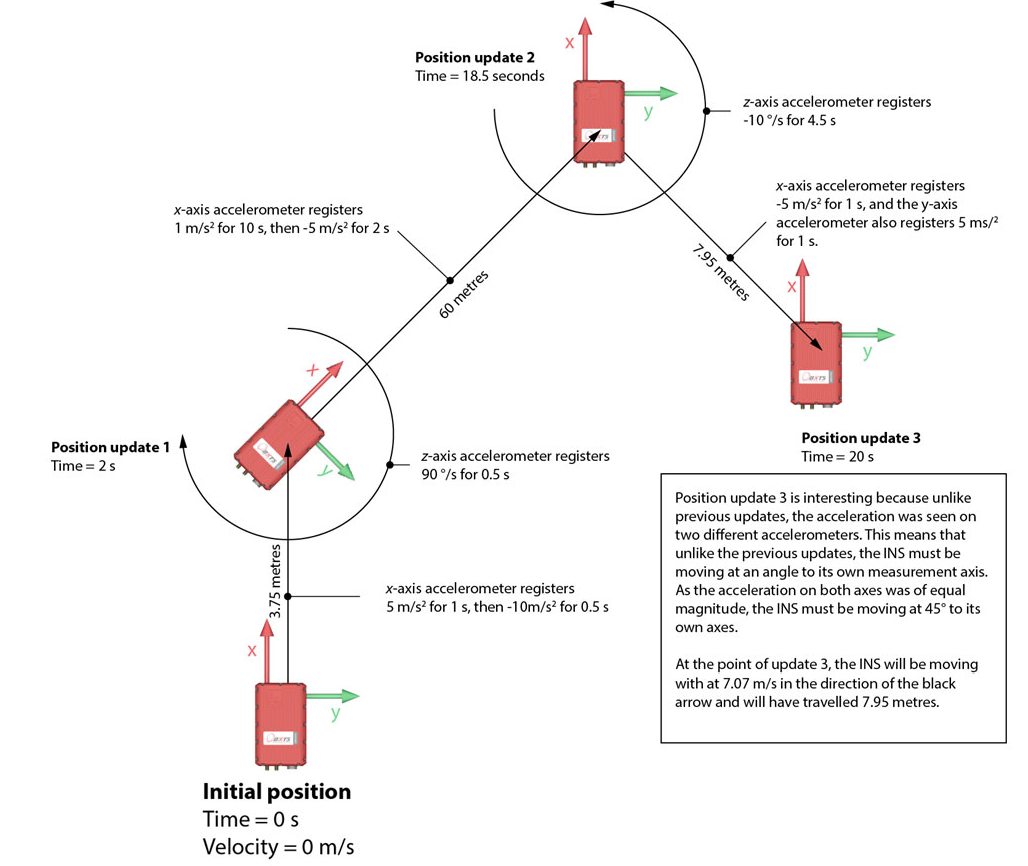
\includegraphics[scale=0.45]{gambar/Dead-reckoning-INS.png}
  % Keterangan gambar yang diinputkan
  \caption{\emph{Inertial navigation} menggunakan \emph{Dead Reckoning} \parencite{oxts2020-dr}}
  % Label referensi dari gambar yang diinputkan
  \label{fig:DR}
\end{figure}

\subsection{Recurrent Neural Network (RNN)}

Jaringan saraf berulang (RNN) adalah jenis jaringan saraf tiruan yang sangat cocok untuk memproses data berurutan, seperti teks, audio, atau data deret waktu. \emph{Recurrent Neural Network} dirancang untuk mengingat
input sebelumnya, memungkinkan mereka untuk memahami konteks dan menggunakan pemahaman tersebut untuk memproses input baru. \emph{Recurrent Neural Network} terdiri dari unit yang disebut "sel" yang memproses data 
input dan meneruskannya ke sel berikutnya dalam jaringan. Sel-sel dalam RNN terhubung dalam satu lingkaran, yang memungkinkan mereka memproses data dalam beberapa langkah waktu. Hal ini membuat RNN sangat berguna 
untuk tugas-tugas seperti terjemahan bahasa atau pengenalan suara, di mana arti sebuah kata atau frase tergantung pada konteks yang diberikan oleh kata atau frase yang datang sebelumnya. Ada beberapa jenis \emph{Recurrent Neural Network}, 
termasuk jaringan \emph{long Short-term Memory} (LSTM) dan \emph{Gated Recurrent Units} (GRU). Jaringan LSTM dan GRU dirancang untuk mengatasi masalah hilangnya dan meledaknya gradien yang dapat terjadi saat melatih
\emph{Recurrent Neural Network} tradisional pada urutan yang panjang. Masalah ini terjadi karena RNN tradisional kesulitan mempertahankan informasi dari langkah waktu sebelumnya saat mereka memproses data melalui 
beberapa langkah waktu. Jaringan LSTM dan GRU keduanya menggunakan mekanisme khusus untuk menyimpan informasi ini dengan lebih baik dan membuatnya lebih mudah untuk melatih \emph{Recurrent Neural Network} pada urutan yang panjang.

Jaringan saraf berulang memori jangka pendek (LSTM) adalah jenis jaringan saraf tiruan yang sangat cocok untuk memproses data berurutan dan mengingat informasi dalam jangka waktu yang lama. varian dari jenis jaringan
saraf berulang (RNN) yang lebih umum, yang dirancang untuk memproses data berurutan dengan memproses data selama beberapa langkah waktu. \emph{long Short-term Memory} (LSTM) sangat berguna untuk tugas-tugas seperti terjemahan bahasa atau 
pengenalan ucapan, di mana arti kata atau frasa bergantung pada konteks yang diberikan oleh kata atau frasa sebelumnya. \emph{long Short-term Memory} (LSTM) juga digunakan dalam aplikasi lain yang penting untuk mengingat informasi dalam 
jangka waktu yang lama, seperti prediksi pasar saham atau terjemahan mesin. Salah satu fitur utama \emph{long Short-term Memory} (LSTM) adalah penggunaan "gerbang", yang digunakan untuk mengontrol aliran informasi 
melalui jaringan. Gerbang dalam jaringan \emph{long Short-term Memory} (LSTM) memungkinkannya menyimpan atau melupakan informasi secara selektif, dan memperbarui keadaan internalnya berdasarkan input yang diterimanya.
Hal ini membuat \emph{long Short-term Memory} (LSTM) sangat efektif dalam belajar dari rangkaian data yang panjang dan mengingat informasi penting dalam jangka waktu yang lama. \parencite{Sak2014}

\emph{Gated Recurrent Units} (GRU) adalah jenis jaringan syaraf tiruan yang cocok untuk memproses data sekuensial, seperti teks, audio, atau data deret waktu. Varian dari jenis jaringan saraf berulang (RNN) yang 
lebih umum, yang dirancang untuk memproses data berurutan dengan memproses data dalam beberapa langkah waktu. \emph{Gated Recurrent Units} (GRU) terdiri dari unit-unit yang disebut "sel", yang memproses data input 
dan meneruskannya ke sel berikutnya dalam jaringan. Sel-sel dalam \emph{Gated Recurrent Units} (GRU) terhubung dalam satu lingkaran, yang memungkinkan mereka memproses data dalam beberapa langkah waktu dan menyimpan 
informasi dari langkah waktu sebelumnya. \emph{Gated Recurrent Units} (GRU) sangat berguna untuk tugas-tugas seperti terjemahan bahasa atau pengenalan ucapan, di mana arti kata atau frasa bergantung pada konteks 
yang disediakan oleh kata atau frasa sebelumnya. GRU juga digunakan dalam aplikasi lain yang penting untuk mengingat informasi dalam jangka waktu yang lama, seperti prediksi pasar saham atau terjemahan mesin. Salah 
satu fitur utama \emph{Gated Recurrent Units} (GRU) adalah penggunaan "gerbang", yang digunakan untuk mengontrol aliran informasi melalui jaringan. Gerbang di \emph{Gated Recurrent Units} (GRU) memungkinkannya 
menyimpan atau melupakan informasi secara selektif, dan untuk memperbarui status internalnya berdasarkan input yang diterimanya. Hal ini membuat \emph{Gated Recurrent Units} (GRU) sangat efektif dalam belajar dari 
rangkaian data yang panjang dan mengingat informasi penting dalam jangka waktu yang lama. \parencite{Dey2017}

Untuk melakukan \emph{Dead Reckoning} menggunakan \emph{Recurrent Neural Network}, jaringan perlu dilatih pada kumpulan data input yang terdiri dari posisi kendaraan sebelumnya dan data sensorik yang dikumpulkan 
selama periode waktu tertentu, dan label output yang sesuai yang mewakili posisi kendaraan saat ini. \emph{Recurrent Neural Network}  kemudian akan dapat membuat prediksi tentang posisi kendaraan saat ini 
berdasarkan data input baru yang terdiri dari posisi kendaraan sebelumnya dan data sensorik yang dikumpulkan pada titik waktu tertentu.Ada banyak aplikasi potensial untuk menggunakan \emph{Recurrent Neural Network}  
untuk perhitungan mati, termasuk kendaraan otonom, drone, dan robot seluler lainnya.Kemampuan untuk secara akurat memperkirakan posisi kendaraan saat ini berdasarkan posisi sebelumnya dan data sensorik dapat sangat 
penting untuk navigasi dan lokalisasi di lingkungan di mana sinyal GPS mungkin tidak tersedia atau tidak dapat diandalkan \parencite{Albawi2017}. 

\subsection{Accelerometers}

Akselerometer adalah otomatis alat untuk mengukur akselerasi, mendeteksi dan mengukur getaran (vibration) dan akselerasi pengukuran karena tubuh (inclination). Akselerometer dapat 
digunakan untuk mengukur getaran pada mobil, mesin, bangunan, dan keamanan Instalasi. Akselerometer juga dapat diterapkan pada mengukur peralatan elektronik, seperti 3 dimensi permainan, 
mouse komputer dan telepon dan gempa bumi kegiatan dan dapat digunakan untuk keperluan multimedia seperti VOD (Video on Demand) yang video tersebut menggunakan gerakan 3D dan objek 3D 
dapat diubah menjadi gambar seperti JPG yang memiliki fungsi kontinu dari intensitas cahaya di sebuah dimensi. Hadir dalam bentuk sirkuit sederhana untuk perangkat elektronik besar. 
Meskipun penampilannya sederhana, akselerometer terbuat dari berbagai bagian dan bekerja dalam banyak hal, dua di antaranya adalah \emph{Capacitance Accelerometer} 
dan \emph{Piezoelectric Acceleromete} \parencite{Randell2003}. 

Untuk sistem akselerometer multi-sensor, pengklasifikasi pohon keputusan digunakan sebagai algoritma klasifikasi. Ukuran jendela tetap 1 sec dan laju pengambilan sampel 20Hz diadopsi untuk sistem ini seperti yang dijelaskan sebelumnya. Untuk pengklasifikasi, mean, var, 
dan \emph{Spectral Energy} diadopsi sebagai fitur karena kemampuan pengenalannya yang lemah. Dua kombinasi fitur masing-masing digunakan untuk pengklasifikasi pohon keputusan: Hanya rata-rata
dan kombinasi mean dan var. Untuk sistem akselerometer sensor tunggal, ukuran jendela tetap 0,5 sec dan frekuensi pengambilan sampel 50Hz diadopsi, karena sistem sensor tunggal lebih 
sensitif terhadap frekuensi pengambilan sampel di bawah 50Hz. Pengklasifikasi dan fitur-fiturnya dipilih berdasarkan studi yang ditentukan Akselerometer sering kali dilengkapi dengan 
rentang pengukuran yang dapat diprogram. Mereka biasanya memiliki minimum rentang pengukuran gaya ±2 g dan naik ke rentang pengukuran gaya ±24 g. Namun memilih rentang pengukuran yang 
tinggi tidak berarti itu akan menjadi pilihan ideal untuk setiap tugas. Ini adalah karena mengonfigurasi akselerometer ke rentang pengukuran yang lebih besar mengurangi presisi 
akselerometer. Karena itu, jika lebih penting bagi suatu tugas untuk dapat mengukur pengukuran yang luas rentang, maka akselerometer akan dikonfigurasi ke rentang pengukuran tertinggi.

\subsection{Magnetometers}

Modul kompas elektronik 3-sumbu sedang dirancang untuk tujuan penginderaan magnetik medan rendah yang memiliki antarmuka digital, untuk tujuan memberikan informasi judul untuk proyek 
mikrokontroler. Sensor ringkas ini biasanya cocok dengan proyek-proyek kecil seperti UAV dan sistem navigasi robot. Sensor sebenarnya mengubah segala jenis medan magnet menjadi output 
tegangan diferensial pada 3 sumbu. Perubahan tegangan ini adalah nilai output digital mentah, yang dapat digunakan untuk tujuan menghitung heading atau merasakan medan magnet yang datang 
dari berbagai arah. Pertumbuhan pasar kompas elektronik 3 sumbu sangat bergantung pada pertumbuhan pasar otomotif dan kedirgantaraan dan pertahanan secara keseluruhan secara global. 
Magnetometer digunakan dalam berbagai aplikasi, termasuk navigasi, pemetaan medan geomagnetik, dan deteksi logam. Dalam sistem navigasi, magnetometer 3 sumbu dapat digunakan untuk 
mengukur medan magnet bumi dan menentukan orientasi perangkat relatif terhadap kutub utara magnet bumi. Ini berguna untuk menentukan arah atau arah perjalanan kendaraan atau perangkat, 
terutama dalam situasi di mana sinyal GPS tidak tersedia atau tidak dapat diandalkan.

Terlepas dari banyak faktor pendorong, pasar kompas elektronik 3-sumbu diperkirakan akan menunjukkan menyusut dan fluktuasi tingkat pertumbuhan karena adanya teknologi GPS sebagai 
pengganti aplikasi serupa yang terkait dengan navigasi. Tidak adanya perangkat keras tambahan untuk e-compass atau kompas navigasi bertindak sebagai faktor penahan untuk pasar kompas 
elektronik 3-sumbu global. Pengurangan paket sensor untuk tujuan mengintegrasikannya secara efisien ke dalam produk elektronik portabel telah secara portentous mendorong pertumbuhan 
pasar kompas elektronik 3-sumbu dalam beberapa waktu terakhir dan akan menciptakan peluang yang signifikan untuk kompas elektronik 3-sumbu di tahun-tahun mendatang. Ada beberapa jenis 
magnetometer, termasuk fluxgate, efek hall. Magnetometer Fluxgate menggunakan gulungan kawat yang dikelilingi oleh inti feromagnetik. Ketika 
medan magnet hadir, inti termagnetisasi, yang menyebabkan perubahan resistansi kawat. Magnetometer efek hall menggunakan magnetometer tipis, konduktor datar yang diposisikan dalam medan 
magnet. Ketika arus dilewatkan melalui konduktor, dihasilkan tegangan yang sebanding dengan kekuatan medan magnet. Magnetometer yang dipompa secara optik menggunakan laser untuk mengukur 
penyerapan cahaya oleh spesies atom atau molekul untuk menentukan kekuatan medan magnet.

\subsection{Gyroscope}

Giroskop adalah perangkat yang dipasang ke bingkai dan dapat merasakan kecepatan sudut jika itu bingkai adalah rotasi. Ada beberapa kelas giroskop, tergantung pada operasi fisik dan 
teknologi yang melibatkan. Giroskop dapat berdiri sendiri atau digunakan untuk sesuatu sistem yang kompleks, seperti Inertial Measurement Unit (IMU), gyrocompass, sistem referensi judul 
sikap dan sistem navigasi. Untuk mengukur efek Koriolis, giroskop MEMS mengandung massa bergetar yang bergetar di sepanjang drive sumbu. Getaran sekunder diinduksi 
dengan sumbu indera tegak lurus yang menggantikan massa darinya jalur asli ketika giroskop diputar. Prinsip kerja giroskop di mana rotasi di sekitar sumbu masing-masing. 
Giroskop memperkenalkan kapasitansi berubah untuk mendeteksi perpindahan ini. Berbasis pada ini, kecepatan sudut IMU dapat diukur dan dengan mengintegrasikan sinyal, kita dapat memperoleh
orientasi \parencite{Passaro2017}.

Giroskop struktur bergetar mengandung massa mesin mikro yang terhubung ke rumah luar oleh satu set mata air. Rumah luar ini terhubung ke papan sirkuit tetap oleh set pegas ortogonal 
kedua. Massa terus menerus didorong sinusoidal di sepanjang set pegas pertama. Setiap rotasi sistem akan menginduksi percepatan Koriolis dalam massa, mendorongnya ke arah set pegas 
kedua. Ketika massa diusir dari sumbu rotasi, massa akan didorong tegak lurus dalam satu arah, dan ketika didorong kembali ke arah sumbu rotasi, ia akan didorong ke arah yang 
berlawanan, karena gaya Koriolis yang bekerja pada massa.


  \newpage

  % Konten metodologi
  \chapter{METODOLOGI}

% Ubah konten-konten berikut sesuai dengan isi dari metodologi

\section{Metode yang digunakan}

% Ubah paragraf berikut sesuai dengan METODE YANG DIGUNAKAN dari tugas akhir
% Contoh input gambar dengan format *.jpg
\begin{figure} [ht] \centering
  % Nama dari file gambar yang diinputkan
  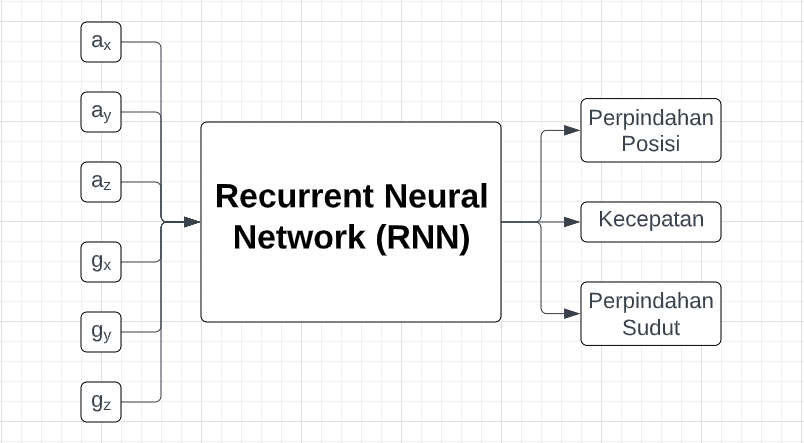
\includegraphics[scale=0.35]{gambar/RNN-3Dimensi.png}
  % Keterangan gambar yang diinputkan
  \caption{Pemrosesan data jarak yang ditempuh pada RNN}
  % Label referensi dari gambar yang diinputkan
  \label{fig:RNN-3D}
\end{figure}

Dengan menerapkan sistem \emph{Pose and Position} dalam dua dimensi (x,y) maka dari itu data yang dihasilkan pada nilai 3-Sumbu \emph{Gyroscope} 
yang memperoleh sumbu Az dan Gz tidak diperlukan karena jika dipakai, dibutuhkan setidaknya tiga dimensi (x,y,z) pada objek target.

% Contoh input gambar dengan format *.jpg
\begin{figure} [ht] \centering
  % Nama dari file gambar yang diinputkan
  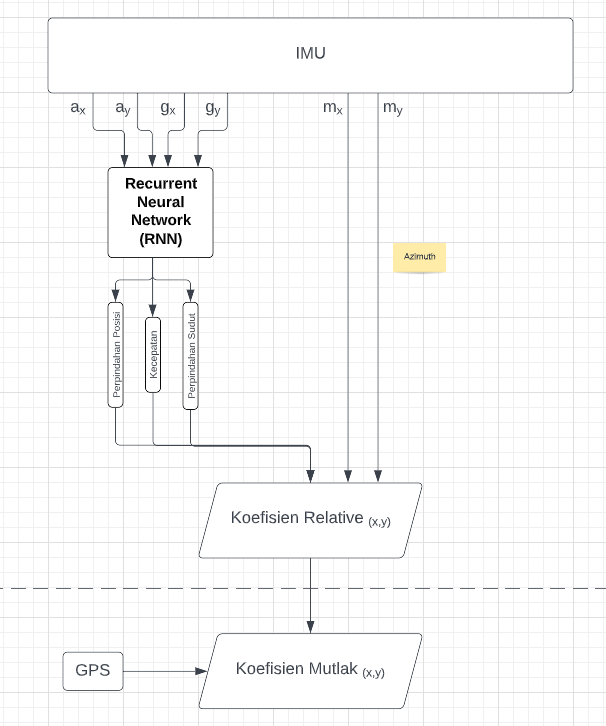
\includegraphics[scale=0.55]{gambar/IMU-to-KRel-KMut.png}
  % Keterangan gambar yang diinputkan
  \caption{Flowchart menentukan Koef. Relatif dengan RNN}
  % Label referensi dari gambar yang diinputkan
  \label{fig:Koef-Relatif}
\end{figure}

% Contoh penggunaan referensi dari gambar yang diinputkan
Pada \emph{flowchart} yang tertera di Gambar \ref{fig:Koef-Relatif} untuk mendapatkan posisi kendaraan memerlukan beberapa tahapan, mulai dari merangkai
seluruh alat-alat yang hendak digunakan untuk pengambilan data. Alat pengujian yang berupa mikrokontroller dengan sensor IMU dan beberapa komponen \emph{Electrical Wiring} 
akan dipasangkan pada kendaraan bermotor, Selanjutnya persiapkan dan instalasi beberapa \emph{Software} pendukung yang dibutuhkan dalam penelitian seperti,
kalibrasi sensor \emph{Inertial Measurement Unit} dengan \emph{Global Position System}, hingga instalasi mikrokontroller STM.  

\section{Bahan dan peralatan yang digunakan}

\subsection{Mikrokontroller STM32}
% Ubah paragraf berikut sesuai dengan Mikrokontroller STM32 dari tugas akhir
Mikrokontroler STM adalah rangkaian mikrokontroler yang dikembangkan dan diproduksi oleh STMicroelectronics, sebuah perusahaan semikonduktor global yang berbasis di Eropa. 
Mikrokontroler STM banyak digunakan dalam berbagai aplikasi termasuk elektronik konsumen, otomotif, kontrol industri, dan sistem komunikasi. Biasanya diprogram menggunakan 
bahasa pemrograman tingkat tinggi seperti C atau C++, dan dapat diprogram menggunakan berbagai alat pengembangan dan lingkungan pengembangan terintegrasi (IDE). 
Mikrokontroller ini juga menyediakan serangkaian pustaka dan alat perangkat lunak untuk membantu pengembang membuat aplikasi untuk mikrokontroler mereka. Seri STM32 didasarkan pada inti ARM Cortex-M3 yang dirancang khusus untuk aplikasi tertanam yang membutuhkan kinerja tinggi, biaya rendah, dan konsumsi daya rendah. Ini dibagi menjadi 
produk yang berbeda sesuai dengan arsitektur inti: Di antara mereka, seri STM32F meliputi: seri "ditingkatkan" STM32F103, seri "dasar" STM32F101, STM32F105, seri "interkoneksi" STM32F107, 
dan seri yang ditingkatkan dengan frekuensi clock 72MHz, yang merupakan produk kinerja tertinggi di antara produk serupa. 

% Contoh input gambar dengan format *.jpg
\begin{figure} [ht] \centering
  % Nama dari file gambar yang diinputkan
  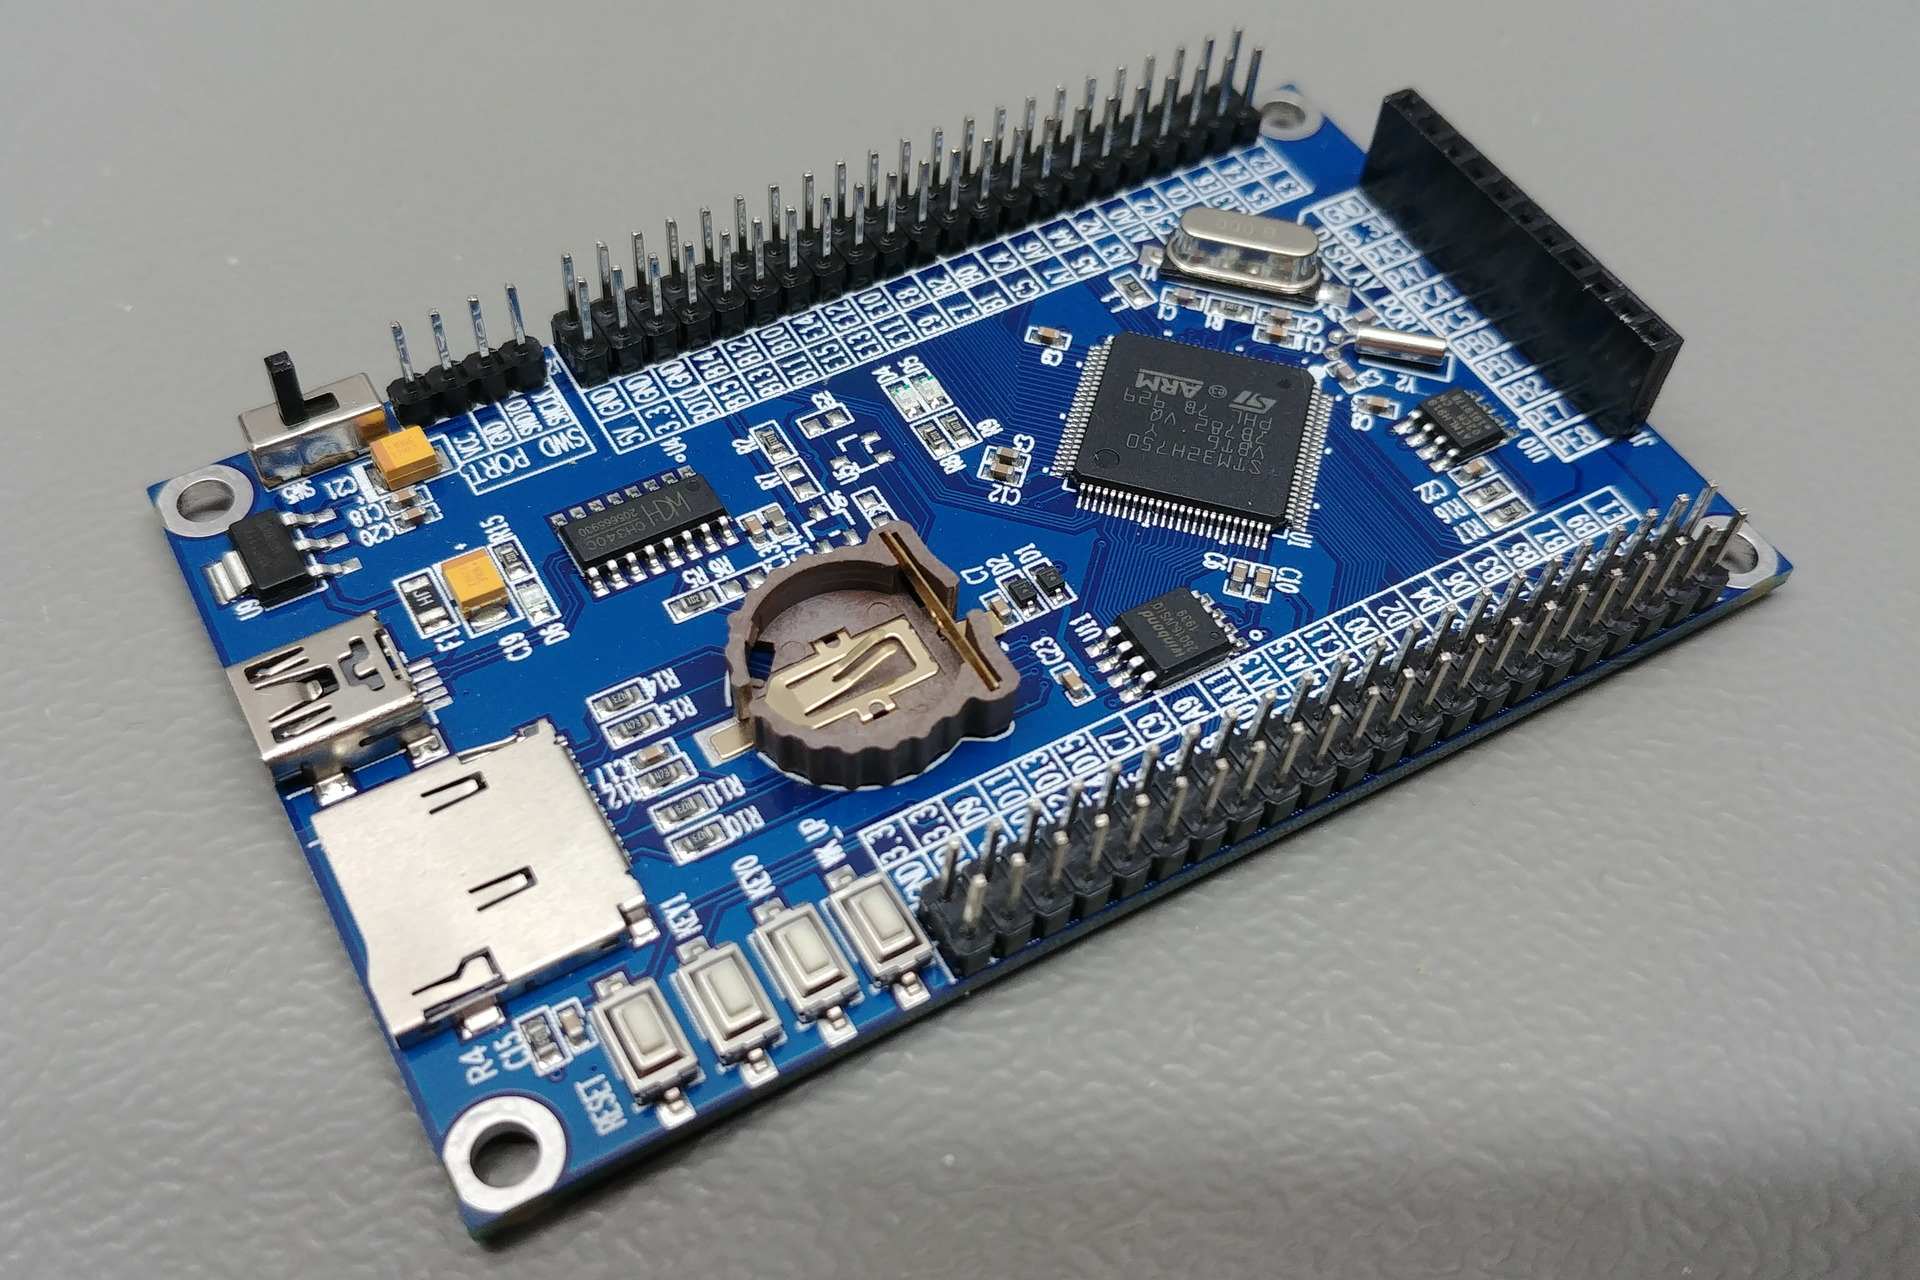
\includegraphics[scale=0.35]{gambar/STM32H750VBT6_Generic_Development_Board.jpg}
  % Keterangan gambar yang diinputkan
  \caption{ST-Microelectronics STM32H750VBT6, Arm Cortex-M7}
  % Label referensi dari gambar yang diinputkan
  \label{fig:STM-Board}
\end{figure}

\subsection{IMU Sensor Module MPU-9255}
% Ubah paragraf berikut sesuai dengan SENSOR MODULE IMU dari tugas akhir
MPU-9255 adalah \emph{Inertial Measurement Unit} (IMU) 9-sumbu yang dikembangkan oleh InvenSense, sebuah perusahaan yang berspesialisasi dalam desain dan pembuatan pelacakan gerak dan sensor 
pencitraan. MPU-9255 adalah perangkat kecil berdaya rendah yang dapat mengukur akselerasi, laju sudut, dan medan magnet dalam tiga dimensi. Ini umumnya digunakan dalam aplikasi seperti 
drone, robotika, realitas virtual, dan teknologi yang dapat dikenakan untuk memberikan informasi waktu nyata tentang orientasi, gerakan, dan akselerasi perangkat. 
Untuk menggunakan MPU-9255, Anda harus menghubungkannya ke mikrokontroler atau perangkat lain yang dapat berkomunikasi dengannya menggunakan antarmuka digital seperti I2C atau SPI. 
Nantinya kemudian perlu menulis kode untuk membaca data dari MPU-9255 dan menginterpretasikannya berdasarkan persyaratan aplikasi spesifik. InvenSense menyediakan serangkaian 
pustaka dan alat perangkat lunak untuk membantu pengembang membuat aplikasi menggunakan MPU-9255.

% Ubah paragraf berikut sesuai dengan PC/HP dari tugas akhir
\section{Urutan pelaksanaan penelitian}

% Ubah tabel berikut sesuai dengan isi dari rencana kerja
\newcommand{\w}{}
\newcommand{\G}{\cellcolor{gray}}
\begin{table}[h!]
  \begin{tabular}{|p{3.5cm}|c|c|c|c|c|c|c|c|c|c|c|c|c|c|c|c|}

    \hline
    \multirow{2}{*}{Kegiatan} & \multicolumn{16}{|c|}{Minggu} \\
    \cline{2-17} &
    1 & 2 & 3 & 4 & 5 & 6 & 7 & 8 & 9 & 10 & 11 & 12 & 13 & 14 & 15 & 16 \\
    \hline

    % Gunakan \G untuk mengisi sel dan \w untuk mengosongkan sel
    Studi pustaka &
    \G & \G & \G & \w & \w & \w & \w & \w & \w & \w & \w & \w & \w & \w & \w & \w \\
    \hline

    Perancangan alat dan Pengambilan data &
    \w & \G & \G & \G & \w & \w & \w & \w & \w & \w & \w & \w & \w & \w & \w & \w \\
    \hline

    Pengolahan data dan Pembuatan struktur model &
    \w & \w & \w & \w & \G & \G & \G & \G & \w & \w & \w & \w & \w & \w & \w & \w \\
    \hline

    Training, Validasi dan Pengujian Dataset &
    \w & \w & \w & \w & \w & \w & \G & \G & \G & \G & \w & \w & \w & \w & \w & \w \\
    \hline

    Penerapan model dan Penganalisaan hasil data &
    \w & \w & \w & \w & \w & \w & \w & \w & \G & \G & \G & \G & \w & \w & \w & \w \\
    \hline

    Perhitungan perbedaan K.Relatif (tanpa GPS) dengan K.Mutlak (dengan GPS) &
    \w & \w & \w & \w & \w & \w & \w & \w & \w & \w & \w & \w & \G & \G & \G & \w \\
    \hline

    Evaluasi penelitian &
    \w & \w & \w & \w & \w & \w & \w & \w & \w & \w & \w & \w & \w & \w & \G & \G \\
    \hline

    Penyusunan laporan &
    \G & \G & \G & \G & \G & \G & \G & \G & \G & \G & \G & \G & \G & \G & \G & \G \\
    \hline

  \end{tabular}
  \captionof{table}{Tabel timeline}
  \label{tbl:timeline}
\end{table}

Pada \emph{timeline} yang tertera di Tabel \ref{tbl:timeline}, terdapat 16 minggu pengerjaan penelitian, 
mulai dari satu bulan pertama ada Studi pustaka dengan Perancangan alat dan Pengambilan data, 
bertujuan untuk mengkaji ulang sedikit literatur yang kurang sesuai pada Proposal Tugas Akhir dan mulai 
merancang alat. dua bulan setelahnya adalah Pengolahan data dan Pembuatan model, serta Penerapan model dan 
Penganalisaan hasil data yang diperoleh. Di empat bulan terakhir adalah penambahan sedikit fitur atau mengetahui 
perbedaan antara dua buah obyek dengan substansi yang berbeda, jika ditemukan beberapa kesalahan dataset serta modeling 
bisa dilakukan evaluasi secara cepat.
  \newpage

  % Konten lainnya
  \chapter{HASIL YANG DIHARAPKAN}

\section{Hasil yang Diharapkan dari Penelitian}

Dari penelitian yang akan dilakukan, diharapkan \lipsum[15]

\section{Hasil Pendahuluan}

Sampai saat ini, kami telah \lipsum[16]

  \newpage

  % Daftar pustaka
  \chapter*{DAFTAR PUSTAKA}
  \addcontentsline{toc}{chapter}{DAFTAR PUSTAKA}
  \renewcommand\refname{}
  \vspace{2ex}
  \renewcommand{\bibname}{}
  \begingroup
    \def\chapter*#1{}
    \printbibliography
  \endgroup


\end{document}
